\documentclass[../HFT-main.tex]{subfiles}
\begin{document}

\section{Triangle Networks to the Rescue}

The most common objection to the \LINK protocol is that when the link stops, all communication stops.

The solution is to have another path to recover  from -- \emph{not}  the Clos Network, or any "fabric" that you have to go through.

When you have three or more nodes participating in the transaction recovery, you can recover in under a microsecond, without "the fabric" interfering with recovery.

This problem has been discovered, and solved, by the quantum networks community. 

\begin{marginfigure}
  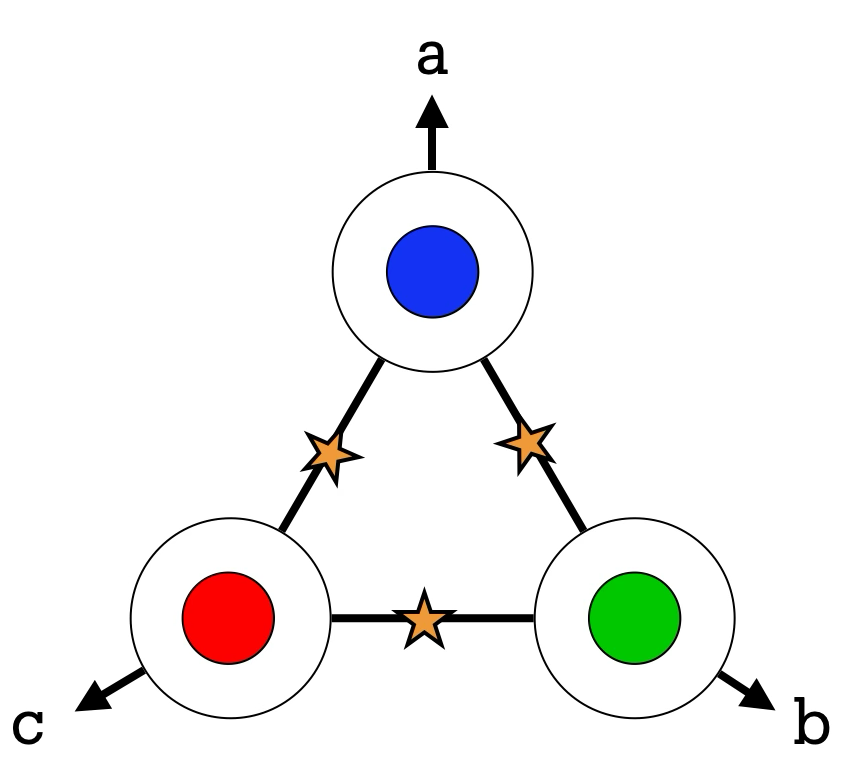
\includegraphics[width=0.5\linewidth]{../Figures/Quantum-Triangle.png}
  \caption{Triangle Networks [Ref]}
    \vspace{25pt}
\end{marginfigure}


Æthernet requires directly connected networks, it will fail if we connect through a switched (Clos) Network instead of connecting directly.\marginnote{It is not possible to achieve reliability through a switch. Temporal intimacy requires immediate link knowledge. We lose Temporal Intimacy, and the paired Shannon Information, when switches Drop, Reorder, Duplicate and delay messages.}

\begin{marginfigure}
  \vspace{20pt}
  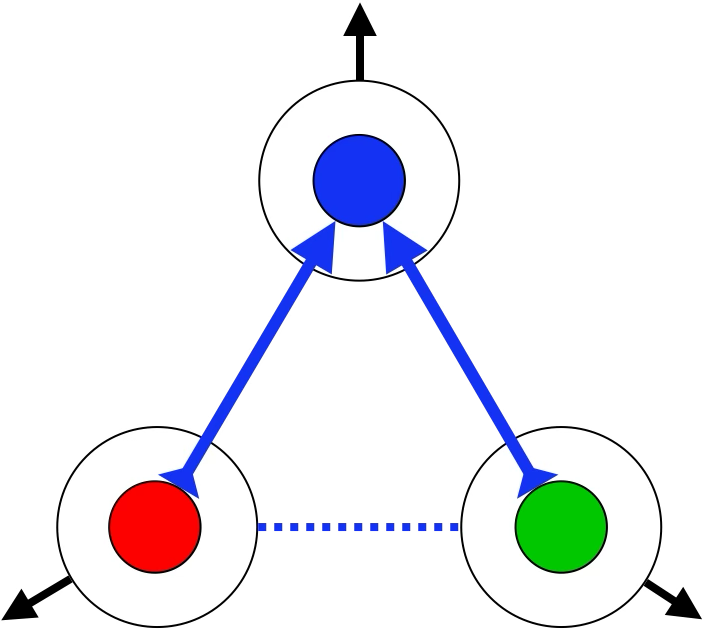
\includegraphics[width=0.5\linewidth]{../Figures/Quantum-Triangle-A.png}
  \caption{Quantum Triangle Tree A}
  \vspace{10pt}
\end{marginfigure}

\begin{marginfigure}
  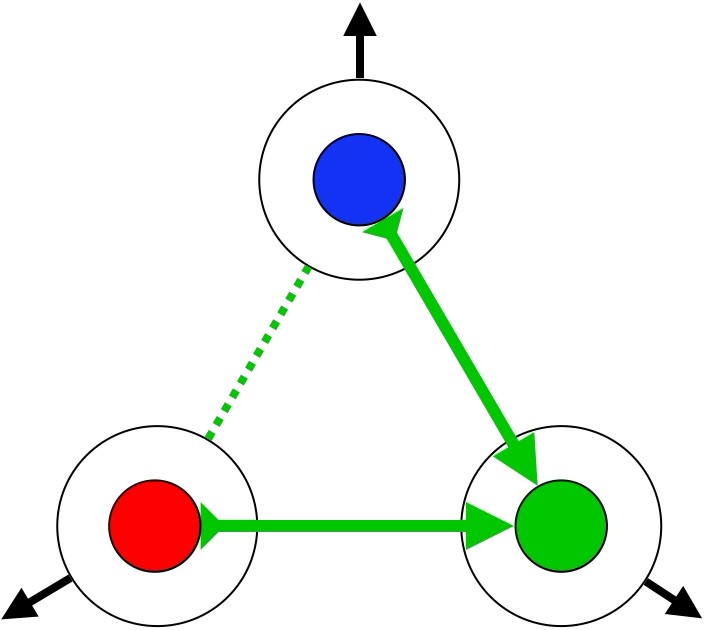
\includegraphics[width=0.5\linewidth]{../Figures/Quantum-Triangle-B.png}
  \caption{Quantum TriangleTree  B}
    \vspace{10pt}
\end{marginfigure}

\begin{marginfigure}
  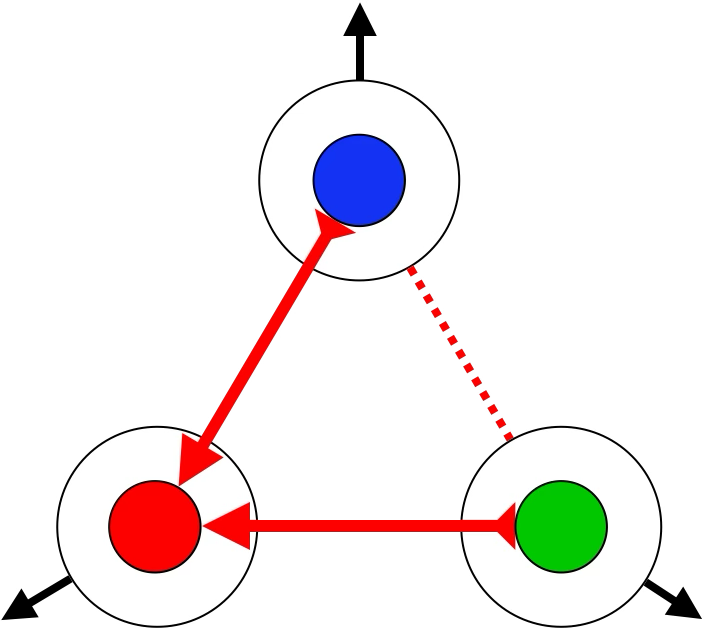
\includegraphics[width=0.5\linewidth]{../Figures/Quantum-Triangle-C.png}
  \caption{Quantum Triangle Tree C}
    \vspace{10pt}
\end{marginfigure}

\subsection{Quantum Networking folks discovered \textbf{Triangle Networks}}

The Æthernet protocol is designed to be exquisitely sensitive to packet loss and corruption.

It can monitor, detect, diagnose link failures, and recover reversibly and automatically \emph{locally} using triangle networks.

%Is it $2^{num edges}$? I'm getting ~4000 partitions and wonder what I'm doing wrong ?
%
%I stopped counting at 1,296, but it can be up to 2,400. From node A's perspective - it can have visibility of BCD, or just BC, BD, CD, B, C, D - which is 7 partitions. The same can simultaneously happen (or not) from B, C, and D's perspective, so that gives us $7^4.$

\begin{itemize}
\item It takes two to tango. It takes three to party.
\item Problem: Status of each link is unknown
\item Use-case: PTP Trees. How do you spot the ``signatures of loss of synchronization''?
\item Solution:  Self-Healing Communication Trees\footnote{\href{https://patentimages.storage.googleapis.com/26/12/fc/a9cee5d1bf69ca/WO2010078506A1.pdf}{Self-Healing Communication Trees (Patented 2005)}}
\item Three Trees (Blue, Green Red) are shown on the right.  Without at least 3 directly connected nodes, it is impossible to guarantee Temporal intimacy, and with it:
	\begin{itemize}
	\item Exactly-Once Semantics
	\end{itemize}
\item IEEE 1588 has 256 Trees
\end{itemize}
keynote

\end{document}